\documentclass{ucalgthes1}   
\usepackage[letterpaper,top=1in, bottom=1.22in, left=1.40in, right=0.850in]{geometry}
\usepackage{fancyhdr}
\fancyhead{}
\fancyfoot{}
\renewcommand{\headrulewidth}{0pt}
\fancyhead[RO,LE]{\thepage}  
\usepackage{hyperref}

\usepackage{algorithm}
\usepackage{algorithmic}
\usepackage{amsfonts}
\usepackage{amssymb}
\usepackage{amsmath}
\usepackage{amsthm}
\usepackage{comment}
\usepackage{float}
\usepackage{graphics}

\theoremstyle{plain}
\newtheorem{thm}{Theorem}[section]
\newtheorem{lemma}[thm]{Lemma}
\newtheorem{prop}[thm]{Proposition}
\newtheorem{cor}[thm]{Corollary}
\theoremstyle{definition}
\newtheorem{defn}[thm]{Definition}

\renewcommand{\algorithmicrequire}{\textbf{Input:}}
\renewcommand{\algorithmicensure}{\textbf{Output:}}

\newcommand{\CC}{\mathbb{C}}
\newcommand{\NN}{\mathbb{N}}
\newcommand{\RR}{\mathbb{R}}
\newcommand{\KK}{\mathbb{K}}
\newcommand{\MM}{\mathcal{M}}
\newcommand{\OO}{\mathcal{O}}
\newcommand{\ZZ}{\mathbb{Z}}
\newcommand{\QQ}{\mathbb{Q}}
\newcommand{\NP}{\textrm{NP}}
\newcommand{\RRgtz}{\mathbb{R}_{>0}}
\newcommand{\ZZgtz}{\mathbb{Z}_{>0}}
\newcommand{\ZZgez}{\mathbb{Z}_{\ge 0}}
\newcommand{\QQgtz}{\mathbb{Q}_{>0}}
\newcommand{\QQgez}{\mathbb{Q}_{\ge 0}}
\newcommand{\matrixto}[2]{\left( \begin{array}{rr} #1 & #2 \end{array} \right)}
\newcommand{\matrixot}[2]{\left( \begin{array}{r} #1 \\ #2 \end{array} \right)}
\newcommand{\matrixtt}[4]{\left( \begin{array}{rr} #1 & #2 \\ #3 & #4 \end{array} \right)}
\newcommand{\ntoinfty}{\lim_{n \rightarrow \infty}}
\newcommand{\floor}[1]{\left\lfloor #1 \right\rfloor}
\newcommand{\ceil}[1]{\left\lceil #1 \right\rceil}

%\setlength{\parindent}{0pt}
%\setlength{\parskip}{2ex} 

\begin{document}

\setcounter{chapter}{2}
\chapter{Exponentiation}

Exponentiation, i.e. computing $g^n$ for some $g$ in a group $G$ and an integer $n$, is useful in many contexts.  Diffie-Hellman key exchange is an example where two parties can jointly establish a shared secret key over an insecure channel. The fundamental operation of Diffie-Hellman key exchange is group exponentiation. Another application discussed in more detail in this thesis is that of computing the order of a group element.  Our approach in this case is to exponentiate a group element to the product, $P$, of several small prime powers.  The result is an element whose order is known to not contain any of these small prime powers. The order of this new element is then computed using a variant of Shanks' baby-step giant-step algorithm where only powers relatively prime to $P$ need to be computed.  Determining the order of an element can be useful in computing the structure of a group, or in factoring an integer that is associated with the group.  In these examples, being able to perform group exponentiation faster means that we can perform a Diffie-Hellman key exchange faster, or that we can compute the order of a group element more quickly.

In Sections \ref{section:binary} and \ref{section:naf} we discuss standard exponentiation techniques that rely on a base 2 representation of the exponent.  The method using non-adjacent form described in Section \ref{section:naf} also benefits when the cost of computing the inverse of a group element is inexpensive or relatively free.  In Section \ref{section:dbns} we introduce double-base number systems, which, as the name implies, are number systems that make use of multiple bases in the representation of a number. In Section \ref{section:dbnsMethods} we discuss some methods to compute double-base representations found in the literature.  In this thesis, we pay particular attention to representations that use bases 2 and 3, since a representation using base 3 can benefit when the cost of cubing an element is less than the cost of multiplying an element with its square.


%%%%%%%%%%%%%%%%%%%%%%%%%
% BINARY EXPONENTIATION %
%%%%%%%%%%%%%%%%%%%%%%%%%
\bigbreak
\section{Binary Exponentiation}\label{section:binary}
The most common and well known method of exponentiation is that of binary exponentation.  This method is often used in Computer Science as an exercise to teach algorithms.  Let $g$ be an element in the group $G$ and $n$ be an integer.  We want to compute $g^n \in G$.  We first represent $n$ in binary as
\[
	n = \sum_{i=0}^{\floor{log_2 n}} b_i 2^i
\]
where $b_i \in \{0, 1\}$ such that $b_i$ represents the $i^{\textrm{th}}$ bit of $n$.   We compute $g^{2^i}$ by repeated squaring of $g$ and compute $g^n$ by computing
\[
	g^n = \prod_{i=0}^{\floor{log_2 n}} g^{b_i 2^i}.
\]
This description is known as right-to-left binary exponentiation as the result is computed by evaluating the bits of the exponent $n$ from right to left.  The left-to-right variant evaluates the bits of the exponent $n$ from left to right by repeatedly squaring the result and multiplying this with the base element $g$ when $b_i = 1$.  The left-to-right variant has the advantage that one of the values in the multiplication remains constant throughout the evaluation, namely $g$.  There also exist windowed variants where $g^w$ is precomputed for each $w$ in some window $0 \le w \le 2^k$ for some $k$ (typically chosen to be cache efficient). The exponent $n$ is then expressed in base $2^k$.  There are numerous sources discussing windowed variants such as (TODO) but, we do not discuss these variants further here.

Binary exponentiation algorithms require on average $\floor{log_2 n}$ squarings and $\floor{log_2 n}/2$ multiplications, since a multiplication is only necessary when $b_i = 1$ and the probability of $b_i = 1$ is 1/2.

%%%%%%%%%%%%%%%%%%%%%%
% NAF EXPONENTIATION %
%%%%%%%%%%%%%%%%%%%%%%
\bigbreak
\section{Non-Adjacent Form Exponentiation}\label{section:naf}

Non-Adjacent Form (NAF) refers to the representation of a number given a \emph{signed} base two representation.  That is, a number $n$ is represented such that
\[
	n = \sum_{i=0}^{\floor{log_2 n}+1} s_i 2^i
\]
where $s_i \in \{0, 1, -1\}$.  As the name suggests, for a number to be in non-adjacent form, there cannot be two non-zero terms adjacent in the representation.  For example, suppose $n = 23814216$.  In a binary representation we have
\begin{equation}\label{eq:binaryEg}
	23814216 = 2^3+2^6+2^{13}+2^{14}+2^{16}+2^{17}+2^{19}+2^{21}+2^{22}+2^{24}
\end{equation}
and in non-adjacent form we have
\begin{equation}\label{eq:nafEg}
	23814216 = 2^3+2^6-2^{13}-2^{15}-2^{18}-2^{20}-2^{23}+2^{25}.
\end{equation}
Similar to the binary case, we compute $g^n$ using
\[
	g^n = \prod _{i=0}^{\floor{log_2 n}+1} g^{s_i 2^i}.
\]
Since $s_i$ may be 0, 1, or -1, non-adjacent form is particularly useful when the cost of computing $g^{-1}$ is relatively inexpensive (or essentially free as in the case of the ideal class group).  However, by computing the product as
\[
	g^n = \left( \prod_{i : s_i=1} g^{2^i} \right) \cdot \left( \prod_{i : s_i=-1} g^{2^i} \right)^{-1}
\]
we can minimize the number of inversions required to at most 1.

There are various methods for evaluating $g^n$ when $n$ is given in non-adjacent form.  As in the binary case, we can compute the evaluation left-to-right, right-to-left, and we can use windowing techniques.  A standard technique is to inspect $n$ from right-to-left two bits at a time.  If the bit pattern at index $i$ is 01, let $s_i = 1$ and subtract $2^i$ from $n$.  If the bit pattern is 11, let $s_i = -1$ and add $2^i$ to $n$.  When the bit pattern is 00 or 10, let $s_i =0$. 

This method can be improved by maintaining a carry flag $c$ \cite[p.4]{Joye2000}.  It works as above, but instead of adding $2^i$ to $n$, we set $c = 1$, and instead of subtracting $2^i$ from $n$, we set $c = 0$.  When inspecting $n$ two bits at a time, we consider the bit pattern $(m+c) \bmod 4$ where $m$ is the two bits of $n$ at index $i$.  The benefit of this method is noticable for \emph{very} large $n$, since the cost of addition and subtraction is reduced from $O(\log n)$ to $O(1)$.  This technique is given in Algorithm \ref{alg:nafR2LImmutable}.  Note that integer computations such as ``$\floor{n/2^i} \bmod 4$'' can be performed by sliding a window of 2 bits size across the binary representation of $n$.

The particular advantage of a non-adjacent form exponentiation over a binary exponentiation is in regards to the number of operations required.  While the binary method required $\floor{\log_2 n}$ squares and on average $\floor{\log_2 n}/2$ multiplications, a non-adjacent form exponentiation requires at most $\floor{\log_2 n}+1$ squares and on average $(\floor{\log_2 n}+1)/3$ multiplications.  To see this, recall that non-adjacent form requires that no two non-zero terms be adjacent.  Consider any two adjacent terms.  With probability 2/3 the first term is non-zero, in which case, the second term must be zero.  With probability 1/3 the first term is zero, in which case, the probability is 2/3 that the second term is non-zero.  This means that 2/3 of the time, 1 of 2 terms will be non-zero, and $1/3 \times 2/3$ of the time, 1 of 2 terms will be non-zero; so the probability of a given term being non zero is 1/3.


%%%%%%%%
% DBNS %
%%%%%%%%
\bigbreak
\section{Double-Base Number Systems}\label{section:dbns}

A significant advantage of non-adjacent form over a binary representation is that on average the number of non-zero terms (the density of the representation) is lower.  This advantage is accentuated when we extend the representation to a signed double-base number system (DBNS).  Binary and non-adjacent form are both a base 2 number system.  In the case of a double base number system, as the name suggests, this is a number system that uses two bases.  This system was first introduced by Dimitrov and Cooklev in \cite{Dimitrov1995}.  Given two coprime integers $p$ and $q$ and some integer $n$, we represent $n$ as the sum and difference of the product of powers of $p$ and $q$,
\begin{equation}\label{eq:generalDbnsForm}
	n = \sum_{i=1}^k s_i p^{a_i} q^{b_i}
\end{equation}
where $s_i \in \{-1, 1\}$ and $a_i, b_i, k \in \ZZgez$.  Since this thesis focuses on exponentiation in the ideal class group, and since we can compute a square with less cost than a multiply and a cube with less cost than a square plus multiply, we will be particularly interested in bases $p=2$ and $q=3$.

As an example of a 2,3 double-base representation, consider the number $n=23814216$ as above.  Given the bases $p=2$ and $q=3$, \emph{one} possible representation of $n$ is
\begin{equation}\label{eq:chainedEg}
	23814216 = 2^3 3^2 -2^{13} 3^2 +2^{15} 3^6.
\end{equation}
The exponentiation of $g^n$ for some $g \in \mathcal G$ is then given by
\[
	g^{23814216} = g^{2^3 3^2 -2^{13} 3^2 +2^{15} 3^6}.
\]
Note that this was just one possible 2,3 representation of the number 23814216 -- there are many.  For example,
\begin{equation}\label{eq:unchainedEg}
	23814216 = 2^3 3^3 - 2^4 3^6 - 2^8 3^5 + 2^{15} 3^6
\end{equation}
is another valid 2,3 representation.  Different representations will trade off cubings for squarings and the best representation for exponentiation will depend on the actual cost of the individual operations.  Later, we shall see some algorithms that take this into account, but many that are designed to either find representations quickly, representations of a special form, or representations with few terms.

Recall, the binary representation \eqref{eq:binaryEg}, non-adjacent form \eqref{eq:nafEg}, and 2,3 double-base representation \eqref{eq:chainedEg} of 23814216 were
\begin{align*}
	23814216 &= 2^3+2^6+2^{13}+2^{14}+2^{16}+2^{17}+2^{19}+2^{21}+2^{22}+2^{24}, & \mbox{\{using binary\}} \\
	23814216 &= 2^3+2^6-2^{13}-2^{15}-2^{18}-2^{20}-2^{23}+2^{25}, & \mbox{\{using NAF\}} \\
	23814216 &= 2^3 3^2 -2^{13} 3^2 +2^{15} 3^6. & \mbox{\{using 2,3 DBNS\}}
\end{align*}
The binary representation had 10 terms, while the non-adjacent form had only 8 terms.  The double-base representation given above contained only three terms.  Note that while a non-adjacent form has in expectation $\floor{\log_2 n}/3$ terms and a binary representation has in expectation $\floor{\log_2 n}/2$ terms, both are bound by $O(\log n)$ in the number of terms.  In the case of 2,3 double-base representations, it was proved in \cite{Ciet2005} that the number of terms is bound by $O(\log n / \log \log n)$.  Therefore, even if there is no known efficient way to compute $g^3$ or $g^2$, given a sufficiently large input, the number of terms and correspondingly the number of operations, will be fewer than either a non-adjacent form exponentiation or a binary exponentiation.  Many algorithms focus on reducing the number of terms in a 2,3 representation for this reason.   Naturally, the cost of a 2,3 double-base exponentiation is even less if the corresponding cost to compute $g^2$ is less than the cost to compute $g \cdot g$, or the cost to compute $g^3$ is less than the cost to compute $g^2 \cdot g$. 


\bigbreak
\subsection{Chains vs. Representations}

\begin{algorithm}[htb!]
\caption{Computes $g^n$ given $n$ as a chained 2,3 representation}\label{alg:expWithChain}
\begin{algorithmic}[1]
\REQUIRE $g \in \mathcal G,$ \\
$n = \sum_{i=1}^k s_i2^{a_i}3^{b_i},$ \\
$s_1,...,s_k \in \{-1, 1\},$ \\
$0 \le a_1 \le ...\le a_k \in \ZZ,$ \\
$0 \le b_1 \le ... \le b_k \in \ZZ.$
\ENSURE $g^n \in \mathcal G$
\STATE $i \gets 1$
\STATE $a \gets 0$ \COMMENT{current power of 2}
\STATE $b \gets 0$ \COMMENT{current power of 3}
\STATE $T \gets g$ \COMMENT{loop invariant: $T = g^{2^a 3^b}$}
\STATE $R \gets 1_{\mathcal G}$ \COMMENT{product of positive exponents}
\STATE $Q \gets 1_{\mathcal G}$ \COMMENT{product of negative exponents}
\WHILE {$i \le k$}
	\WHILE {$a < a_i$}
		\STATE $T \gets T^2$
		\STATE $a \gets a + 1$
	\ENDWHILE
	\WHILE {$b < b_i$}
		\STATE $T \gets T^3$
		\STATE $b \gets b + 1$
	\ENDWHILE
	\IF {$s_i = 1$}
		\STATE $R \gets R \cdot T$
	\ELSE
		\STATE $Q \gets Q \cdot T$
	\ENDIF
	\STATE $i \gets i + 1$
\ENDWHILE
\RETURN $R \cdot Q^{-1}$
\end{algorithmic}
\end{algorithm}

We say that a \emph{partition} of an integer $n$ is an ordered sequence of terms such that the absolute value of successive terms is non-decreasing and the sum of the terms is equal to $n$.  One method to classify algorithms that compute 2,3 representations is by the constraints they placed on the partitioning of $n$.

\begin{defn}
A partition of an integer $n$ is $\emph{chained}$ if any term $x_i$ divides every term $x_j$ for $x_j > x_i$.  For example, a partition of the form $n = x_1 \pm x_2 \pm \cdots \pm x_k$ into distinct integers $x_1,\dots, x_k$ is such that $a_1 ~|~ a_2 ~|~ \cdots ~|~ a_k$.
\end{defn}

\noindent
Note that a binary representation and non-adjacent form are special types of strictly chained partitions, since for any two non-zero terms $s_i$ and $s_j$ where $i < j$ we have $s_i2^i ~|~ s_j2^j$.  The 2,3 representation of $23814216 = 2^3 3^2 - 2^{13} 3^2 + 2^{15} 3^6$ given above is an example of a chained partition, since $2^3 3^2 ~|~ 2^{13} 3^2 ~|~ 2^{15} 3^6$.  Using the constaint that a representation be chained or unchained, we can classify algorithms into those that compute chained representations and those that do not.

The benefit of restricting 2,3 representations to chained representations is the ease with which one can compute $g^n$ when $n$ is given as a chain.  For example $g^{23814216} = g^{2^3 3^2 - 2^{13} 3^2 + 2^{15} 3^6}$ can be computed by first computing $x_1 = g^{2^3 3^2}$, $x_2 = {x_1}^{2^{10}}$, $x_3 = {x_2}^{2^2 3^4}$, and finally $g^{23814216} = \left(x_1 \cdot x_3\right) \cdot \left(x_2\right)^{-1}$.  Algorithm \ref{alg:expWithChain} can be used to compute $g^n$ for $g \in \mathcal G$ and $n$ given as a chained 2,3 representation.  Let $max_a = \max \{a_1,...,a_k\}$ and let $max_b = \max \{b_1,...,b_k\}$, then the cost of algorithm \ref{alg:expWithChain} for a given chain $n$ is $max_a$ squares, $max_b$ cubes, $k-1$ multiplications, and at most one inverse. Because of this ease, many algorithms to find 2,3 representations of numbers constrain the representations to be 2,3 chains.


\bigbreak
\subsection{Exponentiating general 2,3 representations}

Another class of algorithms compute more general 2,3 representations, representations without the constraint that larger terms be divisible by smaller terms.  These algorithms produce representations of the form
\[
	n = \sum_{i=1}^k s_i 2^{a_i} 3^{b_i}
\]
for $s_i \in \{-1, 1\}, a_i, b_i \in \ZZgez$.  This is essentially the same form as \eqref{eq:generalDbnsForm} but for fixed $p$ and $q$.  Given a general 2,3 representation for an integer $n$, M\'{e}loni and Hasan use a modification of Yao's Algorithm \cite[Section 3.2]{Meloni2009} to achieve the same bound on the number of operations as in algorithm \ref{alg:expWithChain}, but with a bound of $O(\min \{max_a, max_b\})$ on the memory used.  Suppose $max_b < max_a$.  We require the terms to be sorted such that $a_k \ge ... \ge a_1$.  The algorithm works by precomputing a table of $T_b = g^{3^b}$ for $0 \le b \le max_b$.  Beginning with the first term $s_i2^{a_i}3^{b_i}$ with the largest $a_i$, it looks up $T_{b_i} = g^{3^{b_i}}$ and multiplies ${T_{b_i}}^{s_i}$ with the running result.  Let $a' = a_i - a_j$ where $a_j$ is the next largest value or 0 if there are no remaining.  It then squares the running result $a'$ times.  The algorithm removes the term $s_i2^{a_i}3^{b_i}$ from the list of terms, and continues in this way with the term with now largest $a_i$.  The algorithm terminates when there are no more terms in the list.  Algorithm  \ref{alg:yaos} gives pseudo-code for this approach and requires $O(max_b)$ memory.  When $max_a < max_b$, we use a related algorithm that requires the terms to be sorted such that $b_k \ge ... \ge b_1$; it precomputes $T_a = g^{2^a}$ for $0 \le a \le max_a$ and works similar to Algorithm \ref{alg:yaos} but with cubing and squaring appropriately swapped.

\begin{algorithm}[htb!]
\caption{Computes $g^n$ given $n$ in 2,3 representation.}\label{alg:yaos}
\begin{algorithmic}[1]
\REQUIRE $g \in \mathcal G,$ \\
$n = \sum_{i=1}^k s_i2^{a_i}3^{b_i},$ \\
$s_1,...,s_k \in \{-1, 1\},$ \\
$a_1 \ge ... \ge a_k \in \ZZgez,$ \\
$b_1,...,b_k \in \ZZgez.$
\ENSURE $g^n \in \mathcal G$
\IF {k = 1}
	\RETURN $g^{2^{a_1} 3^{b_1}}$
\ENDIF
\STATE $max_b \gets \max \{ b_1, ..., b_k \}$.
\STATE $T_b \gets g^{3^b}$ for $0 \le b \le max_b$ \COMMENT{by cubing $max_b$ number of times}
\STATE $a' \gets a_1-a_2$
\STATE $R \gets \left( T_{b_1} \right)^{2^{a'}}$ \COMMENT{by squaring $a_1-a_2$ number of times}
\STATE $i \gets 2$
\WHILE {$i < k$}
	\STATE $R \gets R \cdot {T_{b_i}}^{s_i}$
	\STATE $a' \gets a_i - a_{i+1}$
	\STATE $R \gets R ^ {2^{a'}}$ \COMMENT{by squaring $a_i - a_{i+1}$ number of times}
	\STATE $i \gets i + 1$
\ENDWHILE
\STATE $R \gets R \cdot {T_{b_k}}^{s_k}$
\STATE $R \gets R ^ {2^{a_k}}$ \COMMENT{by squaring $a_k$ number of times}
\RETURN $R$
\end{algorithmic}
\end{algorithm}

As an example, consider \eqref{eq:unchainedEg}, the 2,3 representation $23814216 = 2^3 3^3 - 2^4 3^6 - 2^8 3^5 + 2^{15} 3^6$.  The algorithm first computes $T_b = g^{3^b}$ for $0 \le b \le 6$.  Note that it is sufficient to store only the values of $g^{3^{b_i}}$ that actually occur in terms (in this example, we need only store $T_3$, $T_5$, and $T_6$).  Let $R_j$ represent the partial exponentiation of the $j$ terms with the largest $b_i$ with $g^{2^{a_{j-1}}}$ is factored out.  Let $R_0 = 1_{\mathcal G}$.  In this example, we compute 
\begin{align*}
	R_1 &= \left( T_6 \right)^{2^7} &&\Rightarrow g^{2^7 3^6}, \\
	R_2 &= \left( R_1 {T_5}^{-1} \right)^{2^4} &&\Rightarrow g^{-2^4 3^5 + 2^{11} 3^6}, \\
	R_3 &= \left( R_2 {T_6}^{-1} \right)^{2^1} &&\Rightarrow g^{-2^1 3^6 -2^5 3^5 + 2^{12} 3^6}, \\
	R_4 &= \left( R_3 T_3 \right) ^ {2^3} &&\Rightarrow g^{2^3 3^3 -2^4 3^6 -2^8 3^5 + 2^{15} 3^6},
\end{align*}
% figure of exponentiating 23814216 with unchained representation
\begin{figure}[H]
\centering
\includegraphics{yao1}
\caption{The construction of $2^3 3^3 - 2^4 3^6 - 2^8 3^5 + 2^{15} 3^6$ using algorithm \ref{alg:yaos}.  Steps are executed from left-to-right, top-to-bottom.}
\label{fig:yao1}
\end{figure}
as depicted by figure \ref{fig:yao1}.  The result of the computation is $g^{23814216} = R_4$.  






\bigbreak
\subsection{Encoding of chains/representations}

Chains are often on the fly, no encoding, or delta.

Representations using Yao's....


\pagebreak
\bigbreak
\section{Methods for computing 2,3 Chains/Representations}\label{section:dbnsMethods}

\bigbreak
\subsection{R2L Chains}

\bigbreak
\subsection{L2R Chains (Ostrowski approximation)}

\bigbreak
\subsection{Pruned Trees}





\end{document}

